% \Huge

\section{Information loss and potential recovery}

We studied information loss due to gravitational collapse. Our two main observational probes (CMB and Galaxy surveys) are widely separated by an era from which we have very little information, and which contains such important events as the formation of the first stars and galaxies. It is, therefore, in our interest to find ways of using the data we collect about our Universe today to recover information about the past. These reconstruction techniques have been widely used to recover information on the Baryon Acoustic Peak, but here we look to even smaller scales. Our aim was to test the limits of reconstruction as well as to look at more realistic methods and see how they perform.

In Chapter 2, we proved that some information will never be recovered. To show this, a perfect reconstruction was performed. We measured the density field at the particle positions and used the knowledge of the initial particle positions to reconstruct it. Because we do not (and cannot) measure the density field in an infinity of locations we cannot capture all of its information. This means, no reconstruction is capable of perfectly recovering the primordial density field.
Figure~\ref{fig:3.2} shows the normalized cross spectra of our reconstructed fields with the initial density field (versus the original correlation). Our reconstruction recovers plenty of  intermediate scale information and the two stay correlated to very small scales. However, on these very small scales, they do decorrelate. This information can never be recovered by reconstructing the density field. The plot shows the most amount of information that could ever be recovered from each redshift. In a way, it shows the limit of what we can ever hope to learn about the primordial density field. 

We have also shown that two of the limiting factors in reconstruction are the resolution used and the redshift. Both of these can be improved upon in practice. More and more information is destroyed with the progress of time. By detecting matter further back in time, we increase the amount of information we can recover. On the resolution side, our limitations are the size of galaxies and how many of them we can detect in a certain volume. Galaxies are also biased tracers of matter, so Galaxy Surveys might not be our best option. A very promising future probe is the Square Kilometre Array (SKA).\todo{ref} It will push both boundaries at the same time. Its goal is to detect atomic hydrogen before reionisation (using the 21cm emission). As we are looking much further back in time ($z>10$) and directly at the matter distribution, this probe will lead to incredible advancements in our knowledge of the early Universe.






\section{Future Work}


\begin{figure}
    \centering
    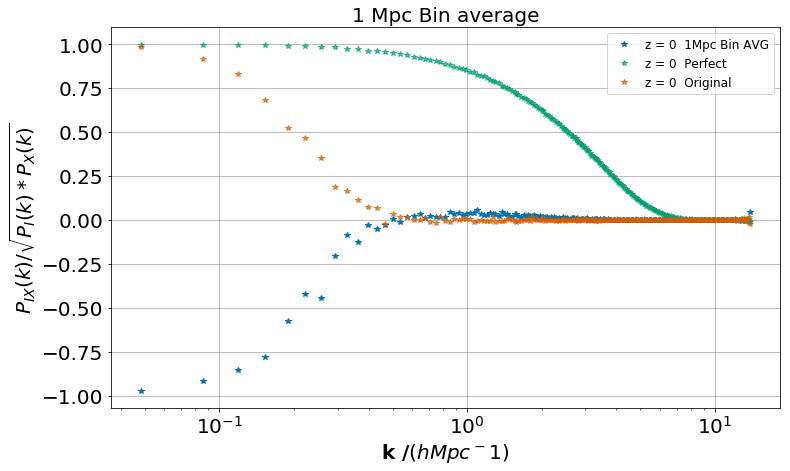
\includegraphics[width=1\columnwidth]{images/realRecon/1MpcBinAvg.png}%
    
    \caption{
        Simulation A reconstruction
    }
    
    \label{fig:12}
\end{figure}

\todo[inline]{Talk about the problems encountered and Future Work.}